% flashcards-title: Cross-product order and normal direction
% flashcards-desc: Vector a points right and vector b points up; an ordered turn and out-of-page and into-page candidates support a right-hand-rule choice.
\documentclass[border=7pt]{standalone}
\def\pgfsysdriver{pgfsys-dvisvgm.def}
\usepackage{tikz}
\usetikzlibrary{arrows.meta,positioning,shapes.geometric}
\definecolor{mechInk}{HTML}{172033}
\definecolor{mechBlue}{HTML}{155EEF}
\definecolor{mechOrange}{HTML}{B54708}
\definecolor{mechPale}{HTML}{E8F0FF}
\definecolor{mechGray}{HTML}{667085}
\definecolor{mechLight}{HTML}{D0D5DD}
\tikzset{
  every picture/.style={font=\sffamily\large, text=mechInk},
  mech box/.style={draw=mechInk, line width=1.2pt, rounded corners=4pt,
    fill=white, align=center, minimum height=14mm, inner xsep=5mm},
  mech primary/.style={draw=mechBlue, line width=2.2pt},
  mech secondary/.style={draw=mechOrange, line width=2.2pt, dashed},
  mech guide/.style={draw=mechGray, line width=0.9pt, dashed},
  mech arrow/.style={-{Stealth[length=3.2mm,width=2.4mm]},
    draw=mechInk, line width=1.4pt, line cap=butt},
  mech axis/.style={draw=mechInk, line width=1.2pt},
  mech tick/.style={draw=mechInk, line width=1pt}
}

\begin{document}
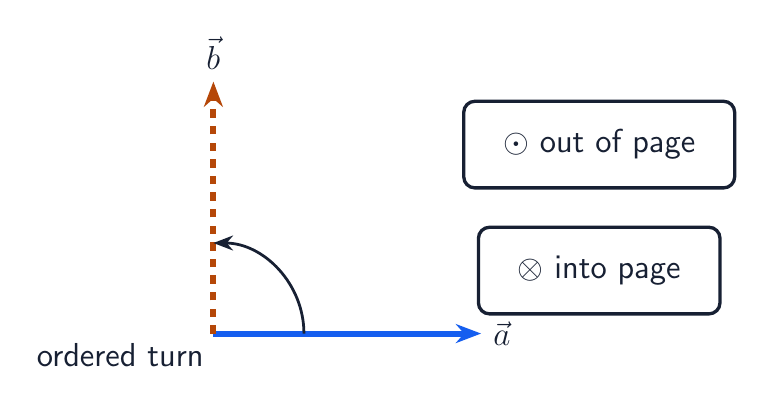
\begin{tikzpicture}[x=1cm,y=1cm]
  \draw[mech primary,-{Stealth[length=3.2mm,width=2.4mm]},line cap=butt] (0,0) -- (3.4,0) node[right] {$\vec a$};
  \draw[mech secondary,-{Stealth[length=3.2mm,width=2.4mm]},line cap=butt] (0,0) -- (0,3.2) node[above] {$\vec b$};
  \draw[mechInk,-{Stealth[length=2.5mm,width=1.9mm]},line width=1pt] (1.15,0) arc[start angle=0,end angle=90,radius=1.15];
  \node[mech box,minimum height=11mm] at (4.9,2.4) {$\odot$ out of page};
  \node[mech box,minimum height=11mm] at (4.9,0.8) {$\otimes$ into page};
  \node[below left] at (0,0) {ordered turn};
\end{tikzpicture}
\end{document}
